\chapter{Basics}
\label{sec:basics}

\section{Machine Learning Overview}

Machine learning is a branch of Artificial Intelligence (AI) that provides systems the ability to automatically learn and improve from experience without being explicitly programmed. Essentially, machine learning involves the creation of algorithms that can learn from and make decisions or predictions based on data. These algorithms work by discovering patterns and insights from data, which is particularly beneficial for decision-making and predictions.

Tom Mitchell provides a classic definition that captures the essence of machine learning: ''A computer program is said to learn from experience E with respect to some task T and some performance measure P, if its performance on T, as measured by P, improves with experience E'' \cite[p. 2]{mitchell1997machine}.

The range of applications for machine learning is extensive, making it an indispensable tool in numerous fields. With today's enormous amounts of data, machine learning is instrumental in harnessing this data for practical use. For instance, in business, it is employed to detect fraudulent activities and gain customer insights. In healthcare, it plays a vital role in identifying trends for improved diagnoses and treatments. Moreover, in the technology sector, it helps refine algorithms and expand the capabilities of AI systems.

Machine learning excels in identifying patterns within data and making predictions based on these patterns. It involves processing data and generating a model that can make inferences from new, unseen data. The accuracy and reliability of these inferences are highly dependent on the quality of the data and the effectiveness of the algorithm used. As a constantly evolving field, machine learning is at the forefront of technological innovation and continues to grow through active research and development.


\subsection{Types of Machine Learning}

Machine learning algorithms can be broadly categorized into three main types based on the nature of the learning signal or feedback available to them during training. The three types are supervised learning, unsupervised learning, and reinforcement learning \cite[p. 10 f.]{ketkar21}.

\subsubsection{Supervised Learning}
Supervised learning is a type of machine learning where the algorithm is trained on a labeled dataset. This means that for every input data, there is a corresponding label or output value associated with it. The algorithm makes predictions or decisions based on this input-output mapping which it learns during the training phase. Once the training is complete, the algorithm can be used to predict output values for new, unseen data. Common algorithms used in supervised learning include linear regression for regression problems and support vector machines, and neural networks for classification problems. Some popular applications of supervised learning include predicting house prices based on various features like size and location, and classifying emails as spam or not spam.

\subsubsection{Unsupervised Learning}
Unlike supervised learning, in unsupervised learning, the algorithm is not provided with labeled data. It tries to learn the patterns and the structure from the data. Clustering and association are two common problems solved by unsupervised learning. Clustering involves grouping data into clusters based on similarity. Dimensionality reduction is another area where unsupervised learning excels. By reducing the number of variables or features, it helps in visualizing multidimensional data, noise reduction, and improving the efficiency of other algorithms. Common algorithms in unsupervised learning include k-means for clustering problems and principal component analysis for dimensionality reduction. It is used in market segmentation, anomaly detection, and recommendation systems among others.

\subsubsection{Reinforcement Learning}
Reinforcement learning is a type of machine learning where an agent learns to behave in an environment by performing certain actions and observing the rewards which it gets from those actions. The goal is to learn a policy that maximizes the expected cumulative reward over time. Unlike supervised learning, there is no correct answer or optimal action that the agent is told. It learns through trial and error. Reinforcement learning has been used in various fields like gaming where it has been used to train agents to play and excel at games like Go and Atari, in robotics for autonomous navigation, and in web-based applications for optimizing click-through rates.

\subsection{Typical Workflow in Machine Learning}
Developing a machine learning model is a systematic process that involves a series of steps. Each step is important for ensuring the reliability and performance of the final model. Below is a summary of the typical workflow in machine learning:

\begin{enumerate}
    \item \textbf{Data Collection:} Gather data relevant to the problem domain in various formats such as tables, images, or text. High quality and relevant data is crucial for training effective models.
    
    \item \textbf{Data Preprocessing and Exploratory Data Analysis (EDA):} Clean the data, handle missing values, normalize features, and encode categorical variables through data preprocessing. Perform EDA to examine the data, understand its characteristics and quality through visualization and statistical analysis.
    
    \item \textbf{Data Splitting:} Divide the data into training, validation, and test sets. The model is trained on the training set, hyperparameters are tuned with the validation set, and the model's performance is evaluated on the test set.
    
    \item \textbf{Model Selection and Training:} Select an appropriate machine learning algorithm based on the nature of the problem and characteristics of the data. Train the model using the training dataset, adjusting its internal parameters to minimize errors.
    
    \item \textbf{Model Evaluation:} Evaluate the model's performance on unseen data using metrics such as accuracy, mean squared error, precision, or recall, depending on the nature of the problem.
    
    \item \textbf{Hyperparameter Tuning:} Optimize the model by adjusting its hyperparameters. Common techniques for hyperparameter tuning include:
    \begin{itemize}
        \item \textbf{Grid Search}: Systematically evaluate all possible combinations of hyperparameters.
        \item \textbf{Random Search}: Randomly sample the space of hyperparameters.
        \item \textbf{Bayesian Optimization}: Use probabilistic models to predict the performance of hyperparameters, selecting promising combinations to evaluate.
    \end{itemize}
\end{enumerate}


\subsection{Challenges in Machine Learning}

Machine learning encompasses a wide array of challenges which are inherent in the nature of the algorithms, the data they work with, and the need to make trade-offs among competing aspects of performance. This section highlights three of the most prominent challenges: overfitting and underfitting, the bias-variance tradeoff, and data quality.

\subsubsection{Overfitting and Underfitting}
Overfitting occurs when a machine learning model captures the noise or random fluctuations in the training data, causing the model to perform poorly on unseen data. This happens because the model becomes too complex and starts to fit not just the underlying trends in the data but also the noise. In contrast, underfitting happens when the model does not capture the underlying trends in the data, usually because it is too simple. Addressing overfitting and underfitting typically involves techniques such as cross-validation, regularization, and using the right complexity in the model.

\subsubsection{Bias-Variance Tradeoff}
The bias-variance tradeoff is a fundamental concept that captures the tradeoff between the model's complexity and its ability to generalize to new data. Bias errors occur when the model makes overly simplistic assumptions about the data, and variance errors occur when the model is too sensitive to small fluctuations in the training data. Striking the right balance between bias and variance is crucial for building a model that performs well on new, unseen data.

\subsubsection{Data Quality}
The performance of a machine learning model is heavily dependent on the quality of the data it is trained on. Low-quality data, which can arise from various issues such as missing values, inconsistencies, and noise, can severely hamper the model's ability to make accurate predictions. Data preprocessing, including cleaning and transformation, is essential for improving data quality before training the model. Furthermore, data augmentation is an effective technique to artificially expand the dataset, especially when the amount of training data is limited. It involves creating new data instances through various modifications of the original data, such as adding noise, scaling, or using synthetic data generation techniques like SMOTE for imbalanced datasets.

\subsection{Introduction to Neural Networks}

Neural networks are computational models inspired by the neural structure of the human brain. They are composed of layers of interconnected processing nodes, known as neurons or artificial neurons. Neural networks have been particularly effective in handling complex and non-linear relationships in data, making them suitable for tasks such as image and speech recognition, natural language processing, and game playing.

\subsubsection{Basic Concepts: Neurons, Weights, and Activation Functions}

A neural network consists of layers of interconnected neurons. Each neuron in a layer is connected to neurons in the previous layer through weighted connections. The fundamental components of neural networks are:

\begin{itemize}
    \item \textbf{Neurons:} The basic processing units of the neural network which compute a weighted sum of their inputs and pass it through a non-linear function, known as an activation function.
    
    \item \textbf{Weights:} These are the values that control the strength and direction of the connection between two neurons. Weights are learned and adjusted during the training process.
    
    \item \textbf{Activation Functions:} These functions introduce non-linearities into the network. Common activation functions include the sigmoid, \ac{tanh}, and \ac{relu}.
\end{itemize}

\subsubsection{Feedforward Neural Networks}

Feedforward neural networks are the simplest type of neural network architecture where the data flows in a single direction from the input layer to the output layer, without any cycles or loops. Each neuron in a layer is connected to every neuron in the previous layer. Feedforward networks are widely used for pattern recognition and are well-suited for mapping input patterns to output patterns \cite[p. 93 f.]{ketkar21}.

\subsubsection{Backpropagation Algorithm}

Backpropagation, short for ''backward propagation of errors'', is a critical algorithm for training neural networks, particularly feedforward neural networks. It is used to minimize the error in the network's predictions by iteratively adjusting the weights and biases. The backpropagation algorithm involves two main phases: the forward pass, where the input is passed through the network to compute the output, and the backward pass, where the gradient of the error with respect to each weight is computed. This gradient information is then used to update the weights in the network to reduce the error \cite[p. 113 ff.]{ketkar21}.


\section{PyTorch Introduction}

PyTorch is an open-source deep learning library developed by Facebook's AI Research lab. It is popular among researchers and developers due to its ease of use, flexibility, and efficient memory usage. PyTorch facilitates the development of deep learning models with its rich set of modules and functionalities. Additionally, PyTorch supports GPU acceleration which can significantly increase the speed of computationally intensive tasks in deep learning \cite[p. 28 ff.]{ketkar21}.

\subsection{Tensors in PyTorch}

Tensors are the fundamental data structures in PyTorch, which generalize the concept of scalars, vectors, and matrices to an arbitrary number of dimensions. They play an important role in building and training deep learning models, as they represent inputs, outputs, and parameters. PyTorch tensors are optimized for GPU processing, which is highly beneficial for computationally intensive tasks.

Creating tensors can be done in multiple ways, such as converting from data like lists or NumPy arrays, or by initializing empty tensors of specific sizes and data types. Furthermore, PyTorch boasts a comprehensive set of operations to manipulate tensors, encompassing arithmetic, linear algebra, matrix manipulation, and sampling, among others. These operations are fundamental for the mathematical computations required in deep learning \cite[Tensors]{pytorch_tutorial}.

\subsection{Datasets and Dataloaders}

Datasets and data loaders are crucial components in data processing and model training in PyTorch. A dataset in PyTorch is an object that contains the data, such as images and labels, which are used for training or testing a model. Dataloaders, on the other hand, efficiently load data from a dataset and offer an easy way to iterate over samples, which is especially helpful for large datasets.

PyTorch provides built-in datasets and data loaders for common tasks like image classification, text analysis, and audio processing. Moreover, users can create custom datasets and data loaders for specific data sources \cite[Datasets and DataLoaders]{pytorch_tutorial}.

\subsection{Transforms}

Data transformation is often necessary to condition the data into a suitable form for training deep learning models. PyTorch's \verb|torchvision.transforms| module provides several common transforms out of the box. Additionally, all TorchVision datasets have two parameters - \verb|transform| to modify the features and \verb|target_transform| to modify the labels - that accept callables containing the transformation logic \cite[Transforms]{pytorch_tutorial}.

\subsection{Building a Neural Network with PyTorch}

PyTorch offers all the building blocks necessary to construct a neural network. Neural networks are made of layers that perform operations on data. In PyTorch, every module subclasses the \verb|nn.Module|. A neural network is itself a module that comprises other modules (layers). 

To define a neural network in PyTorch, one needs to subclass \verb|nn.Module| and initialize the neural network layers in the constructor. The \verb|forward| method is then implemented, which conducts operations on input data.

Neural networks often have parameterized layers, meaning they have associated weights and biases that are optimized during training. These parameters are automatically tracked when a model object subclasses \verb|nn.Module|.

The last linear layer of a neural network usually returns logits, which are raw values ranging from negative infinity to infinity. These logits are then fed through a softmax function to produce probabilities that sum to 1 across specified dimensions \cite[Build Model]{pytorch_tutorial}.

\subsection{Automatic Differentiation with torch.autograd}

PyTorch provides a built-in differentiation engine called \verb|torch.autograd|. It supports automatic computation of gradients for any computational graph. It is a powerful tool that eases the computation of gradients for neural networks, which is essential for the optimization of the weights.

In practice, you only need to declare which tensors you want gradients for by setting \verb|requires_grad=True|. After computing the loss, calling \verb|loss.backward()| will compute the gradients for all tensors with \verb|requires_grad=True|. These gradients are accumulated in the \verb|.grad| attribute of the respective tensors \cite[Automatic Differentiation]{pytorch_tutorial}.

\subsection{Training the Network}

Training a neural network involves iterating over the training data, and for each batch, performing forward and backward passes through the network, computing the loss and updating the weights using an optimization algorithm such as Stochastic Gradient Descent (SGD).

During training, the data is passed through the network (forward pass), and a loss is calculated reflecting how far the network's output is from the ground truth. The gradients of this loss with respect to the network's weights are computed, and the optimizer uses these gradients to update the weights (backward pass) \cite[Optimization Loop]{pytorch_tutorial}.

\subsection{Saving and Loading Models}

Once a model has been trained, it is possible to save its parameters to a file. This is useful for reusing models, sharing them, or deploying them in production environments. In PyTorch, you can use \verb|torch.save()| to save a model's state dictionary, and \verb|torch.load()| to load the state dictionary into a model's architecture.

This process allows for the preservation and later restoration of models, facilitating continuity in research and development, as well as the deployment of machine learning models into production environments \cite[Save, Load and Use Model]{pytorch_tutorial}.


\section{Understanding Ball Bearings}

Ball bearings are mechanical devices that reduce rotational friction and support radial and axial loads. They achieve this by using rolling elements, such as balls, to maintain the separation between the bearing races. This separation minimizes surface contact between the moving parts, thus reducing friction. Ball bearings are vital components in a wide array of machinery and equipment.

\begin{figure}[h]
    \centering
    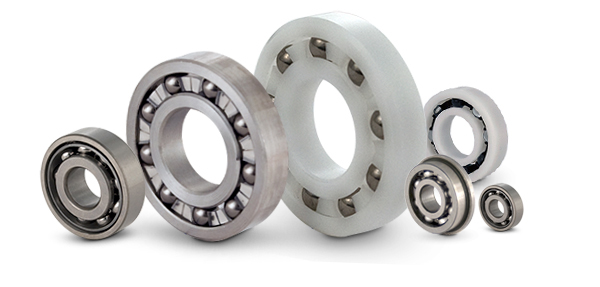
\includegraphics[width=0.5\textwidth]{assets/ball-bearings.jpg}
    \caption{Typical ball bearings \cite{qbcballbearings}}
    \label{fig:ball_bearing}
\end{figure}

\subsection{Components of Ball Bearings}

A typical ball bearing is composed of several fundamental components, including the inner race, the outer race, balls, and a cage. The inner race is a ring that fits tightly on the shaft and has a path on which the balls roll. This race is essential as it rotates with the motion of the shaft. On the other hand, the outer race is similar to the inner race but is larger and remains stationary. It is mounted in the housing and also has a track on which the balls roll. 

The balls themselves are the critical rolling elements within the bearing. These spherical components carry the load and reduce friction as they spin between the inner and outer races. Their smooth surface and round shape are crucial for the free rotation and the distribution of weight.

Another significant component is the cage, sometimes referred to as a retainer. The cage's primary role is to keep the balls evenly spaced around the bearing, preventing them from coming into contact with each other during operation, which could lead to damage or increased friction.

In addition to these primary components, some ball bearings may also include shields and seals. These optional elements are especially useful in environments where contamination from dirt or other particles is a concern, or where there is a need to retain lubricant within the bearing. Shields are generally metal and form a barrier on one or both sides of the bearing, while seals are usually made of rubber and provide a tighter seal to keep out contaminants and hold in lubrication. Both shields and seals contribute to prolonging the bearing's life and maintaining its performance.

\subsection{Functions and Applications of Ball Bearings}

Ball bearings have two primary functions: first, they reduce friction, which is critical for ensuring the smooth rotation of mechanical parts. Second, they support loads, which enables them to sustain both forces perpendicular to the axis of rotation (radial loads) and forces parallel to the axis (axial loads).

In terms of applications, ball bearings are highly versatile. They are found in automotive industry components, including car and truck axles, wheels, and engine parts. In aerospace, they are essential in aircraft engines and systems. Industrial machinery, including motors, pumps, and conveyors, employ ball bearings for efficient operation. Additionally, consumer electronics such as hard drives, DVD players, and fans use ball bearings.


\subsection{Calculating the Lifetime of Ball Bearings}
\label{sec:lifetime_calculation}

Knowing the expected lifetime of ball bearings is essential for minimizing equipment downtime, ensuring reliability, and planning maintenance schedules and budgets. The lifetime of ball bearings depends on the load they bear and the operating conditions. The ISO standard (DIN ISO 281) provides guidelines for calculating the lifetime of ball bearings, differentiating between static and dynamic load capacities.

\subsubsection{Static Load Capacity}
A ball bearing experiences static load when it is either stationary or moving at very low speeds (less than 10 \ac{rpm}). The static load capacity concerns the maximum load that a bearing can sustain without incurring permanent deformation affecting its function. The static load capacity is calculated using the formula:
\begin{equation}
S_{0} = \frac{C_{0}}{P_{0}},
\end{equation}
where \(S_{0}\) is the static load safety factor, \(C_{0}\) is the static load rating, and \(P_{0}\) is the equivalent static bearing load \cite[p. 570 f.]{wittel21}.

\subsubsection{Dynamic Load Capacity}
Dynamic load capacity pertains to a bearing's ability to endure loads while rotating at operational speeds. The lifetime is influenced by fatigue, with the end of life considered when the first signs of material fatigue such as flaking, pitting, or cracks appear on the raceways or balls. The ISO standard defines \(L_{10}\) life as the number of revolutions at which 90\% of a group of identical bearings remain operational. The dynamic load capacity is expressed using the formula:
\begin{equation}
\text{for ball bearings,} \quad L_{10} = \left(\frac{C}{P}\right)^3,
\end{equation}
\begin{equation}
\text{for roller bearings,} \quad L_{10} = \left(\frac{C}{P}\right)^\frac{10}{3},
\end{equation}
where \(L_{10}\) is the bearing life in millions of revolutions, \(C\) is the dynamic load rating, and \(P\) is the equivalent dynamic bearing load. The life in hours (\(L_{10h}\)) is given by:
\begin{equation}
L_{10h} = \frac{10^6}{60 \cdot n} \cdot L_{10},
\end{equation}
where \(n\) is the rotational speed in \ac{rpm} \cite[p. 571 ff.]{wittel21}.

In real-world applications, not all bearings reach the calculated life due to factors such as contamination, poor lubrication, or misalignment. The life calculated is a statistical measure, and in practice, some bearings may fail earlier while others last longer.
